\documentclass{article}
\usepackage{graphicx}
\usepackage{amsmath}
\usepackage{subfig}
\usepackage{float}
\usepackage{caption}
\usepackage[legalpaper, portrait, margin=1in]{geometry}

\title{Analysis of Hydride Structures in Micrographs of Zirconium Samples using Image Processing in Python}
\author{Group 1: S. Khan, A. Hanson, J. Larkin}
\begin{document}
	\maketitle
	
	\begin{center} \textit{This report details progress made during the Research Software \& Engineering in Python module, in which image processing techniques are utilised to automatically analyse micrograph images of zirconium hydride (ZrH) structures in samples of metallic zirconium. The radial hydride fraction (RHF) is computed for a series of micrographs. Explanation of the method, including relevant images and discussion of code elements are included.} \end{center}

\newpage
\tableofcontents
\newpage
	\section{Introduction \& Review of Existing Literature}
	\subsection{Background}
	During the service lifetime of zirconium fuel cladding within a light-water reactor core, several phenomena manifest as a result of both direct neutron irradiation and chemical reactivity with the core coolant. One of the more prominent of these is the formation of zirconium hydride within the bulk material, resulting from the radiolysis of core coolant and subsequent migration of hydrogen through the lattice, which then reacts with the metal and accumulates at grain boundaries. As zirconium hydride is typically more brittle than the lattice itself, this serves to compromise the local integrity of the lattice. 
	\\
	\\
	Zirconium, as a HCP lattice, exhibits a specific crystal \textit{texture} which is determined during component fabrication, the result of which is the alignment of the $<0002>$ basal planes tangentially around the cladding tube. As hydrides typically accumulate parallel to the basal plane, this is advantageous as it prevents the development of cracks radially through the structure which can result in through-wall cracking, compromising the barrier between nuclear fuel and core coolant. Larger scale cracks are able to form due to the close proximity of hydride structures, permitting a brittle fracture through one hydride region to migrate to a neighbouring region, continuing until a large macroscopic crack manifests. This is herein referred to as \textit{hydride connectivity}. One beneficial technique for analysing these phenomena is the use of optical microscopy, which is a widely utilised method for visually assessing micrograph characteristics for specific areas of a sample, including the presence of hydride zones in a metallic matrix (see Figure~\ref{fig:tem_hydride_eg}). Optical microscopy is able to discern structural features with reasonable clarity, however the method does suffer from noise arising from contaminant particles and scratches to the sample surface. In addition, as observed in the sample images used within this study, an 'edge darkening; effect is observed in which pixel intensities appear lower towards the fringes of the image. This presents issues with noise reduction that are discussed later.
	\\
	\begin{figure}[h]
		\centering
		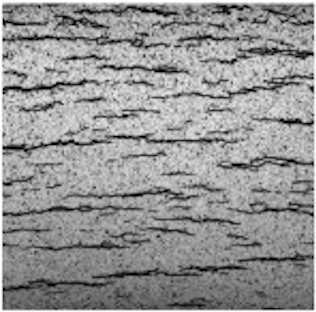
\includegraphics[width=2.5in]{Figures/tem_hydride_eg} 
		\caption{Typical optical micrograph image of darker hydride bands within a zirconium matrix. The horizontal regions are sporadically connected together by small fractures within the material.}
		\label{fig:tem_hydride_eg}
	\end{figure}
	\\
	These micrographs may be processed using appropriate software environments to identify characteristics such as the density of hydride regions within the material, the specific orientations of the hydrides, and the level to which connectivity is observed. Here, image processing techniques within the python programming environment are used to identify these properties, chiefly incorporating the \textit{scikit-image} series of algorithms along with originally-developed scripts. For this project, code is developed, implemented and tested to determine the most effective means of isolating and analysing hydride structures within the images. An account of the evolution of the techniques is given, and results are presented and discussed.
	\\
	\subsection{Literature Review}
	The degradation mechanics of zirconium alloys remain under review as the nuclear sector continues to improve the efficiency and safety of modern nuclear reactors. Research into the degradation of zirconium is a vital component of this research and as such there exists an extensive array of techniques under investigation for accurately predicting this degradation. Practical methods such as x-ray diffraction and resistivity assays are commonplace, however advances in computing power are placing an increased emphasis on the use of computer processing in both independent modelling and comparison with real-world observations.
	\\
	Image processing techniques are utilised for a wide array of different purposes owing to their versatility, reprogrammability and ease of automation. For samples such as micrographs which may exhibit minor differences between images, it is advantageous to automate the process of detecting characteristics to ensure all images are processed identically, therefore reducing systematic errors. In the context of zirconium analysis, several studies have aimed to predict failure routes and lifetime behaviour by quantifying the level and severity of microstructural damage caused by hydride plates evident within sample micrographs, achieved using a range of software packages.
	\\
	\\
	P.A. Simon et al. (2021) \cite{Simon2021} have recently analysed the link between \textit{radial} hydride structures in zirconium and likelihood of eventual failure in MATLAB, and quantified results using a figure known as the \textit{radial hydride continuous path} (RHCP), which considers the geometries of hydride plates, separation distances and the probability of crack propagation through the plates (for which individual regions are assigned a weighting factor). Here, a series of algorithms were used to find the 'best path' for which crack propagation between hydrides is most likely, with micrographs exhibiting more severe crack routes (of greater total length and probability of occurrence) generating a larger value for RHCP (between 0 and 1). The study utilised micrographs of real zirconium samples, binarised and 'cleaned' to remove noise from dust and imperfections within the matrix. It is noted that the complexity of real material micrographs can present issues for many algorithms and as such techniques such as splitting the image into smaller 'bands' are sometimes necessary. The study observed that for higher values of RHCP and r\textit{radial hydride fraction} (RHF), in which greater quantities of radial hydride plates and more crack routes are present, the \textit{fracture energy}, that is, the energy input required for a total fracture to manifest, decreased substantially.
	\\
	RHF as a similar metric to RHCP is used within this study with the similar goal of developing a foundation for predicting the failure modes within zirconium components.
	\\
	\begin{figure}[h]
		\centering
		\subfloat[The crack route through a cladding sample is less 'direct' through the material, as migration between hydride plates is more difficult.]{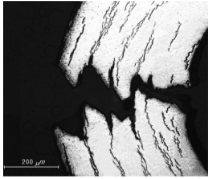
\includegraphics[width=0.45\textwidth]{Figures/circ_frac.PNG}\label{fig:circ_fract}}
		\hfill
		\subfloat[Here, several direct crack routes can be ween in the material owing to a large quantity of radial hydrides, presenting significantly increased probability of through-wall cracking.]{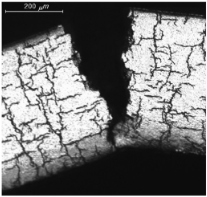
\includegraphics[width=0.4\textwidth]{Figures/rad_frac.PNG}\label{fig:rad_fract}}
		\caption{Micrographs of sections of cladding with varying hydride morphologies observed by P.A. Simon et al. (2021). The fracture route aligns more directly through the material for (b), in which a greater quantity of radially-oriented hydrides are observed. (a) exhibits more circumferentially-aligned hydrides which make crack propagation less favourable \cite{Simon2021}.}
		\label{fig:rad_circ_frac}
	\end{figure}
	\\
    Similarly, the fracture morphologies in oxidised samples of Zircaloy-4 have been investigated by P.A. Raynaud et al. (2012) \cite{RAYNAUD201269}. Here, hydride orientations were characterised using image analysis to assess the effects on the fracture toughness of the cold-worked stress relieved cladding samples. The radial hydride fraction was evaluated by reducing (or 'skeletonising') and indexing all hydride structures along with their corresponding lengths and orientations. Hydrides were further defined as being either 'in-plane', 'mixed' or 'out-of-plane', representing angles of 0-40\textdegree, 40-65\textdegree, and 65-90\textdegree aligned with the hoop direction, respectively. RHF is therefore defined as a weighted average of all indexed hydride lengths and classifications. Overall, increases in RHF throughout the material were found to signifncantly reduce sample fracture toughness. In this study, the radial hydride fraction was evaluated using the Hydromorph software environment.
    \\
    \\
    One more study?
    \\
    \\
    As several previous studies have used various image processing techniques to assess the microstructural characteristics of sample micrographs, it is clear that there is substantial interest in using software to measure metrics relating to the orientation and quantity of hydride plates within metallic matrices. This study attempts to construct an additional route for analysing hydride morphologies using a series of software packages in Python. The primary motivation is the prediction of damage and failure routes in zirconium alloys, which can be qualitatively related to these morphologies and used to determine which samples may be closer to a critical failure than others, and assist in developing our understanding of the effects of hydrides on the structural integrity of fuel cladding elements.
	\\
	\section{Initial Image Processing}
	\subsection{The Gaussian Blur}
	\subsubsection{Gaussian blur theory and approach}
	To begin this project, a series of pre-prepared micrograph images were manipulated and several different approaches in python were tested to provide an initial understanding of the basics of image processing. Algorithms were written which could apply different threshold filters to image value arrays once they had been read into python. When the images were read by the \textit{Scikit image} package in python, they could be expressed as a numerical array with \textit{Numpy}. Threshold values can then be applied to these arrays which can convert an image to binary (black and white) based on the threshold, this requires the image to be converted to greyscale initially.
	\\
	\\
	Although initial scripts succeeded in removing the zirconium matrix and isolating the hydride regions, a significant quantity of noise was observed caused by aberrations in the original images, this may have arised from sample pitting during electropolishing or foreign contaminants on the material or in the microscope used to take the image. As these aberrations manifested at similar pixel intensities to the hydrides themselves, filtering techniques were not able to eliminate them. Therefore, a \textit{blurring} technique was applied prior to intensity filtering in an attempt to remove the noise artefacts.
	\\
	\\
	Here, the function \textit{cv.GaussianBlur()} is utilised, in which a convolution of a Gaussian function is applied to the pixel intensities within a region to be blurred. Although this results in a slight aberration of boundaries for well-defined regions such as hydrides, the effect is minimal due to the relatively large quantities of both black and white pixels either side of the boundary. However, for small scale regions such as several black pixels against a white background (typical of micrograph noise), the technique is highly effective as the small quantity of black pixels tends to disappear when averaged around a large white surround. Figure~\ref{fig:blur_notblur} highlights the removal of artefacts for an initial example micrograph. Upon testing, this technique proved effective for all trialled images.
    
	\begin{figure}[h]
	    \centering
	    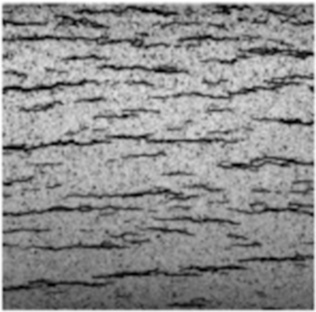
\includegraphics{Figures/blurred_chu1.jpg}
	    \caption{An example of the \textit{Scikit image} gaussian blurring applied to Figure \ref{fig:tem_hydride_eg} with inputs from Table \ref{tab:imageprocessing}}
	    \label{fig:blur_chu1}
	\end{figure}
	
	\begin{figure}[h]
		\centering
		\subfloat[The binarised micrograph without application of Gaussian blurring.]{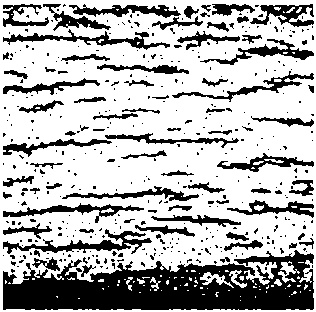
\includegraphics[width=0.4\textwidth]{Figures/not_blurred}\label{blur_notblur1}}
		\hfill
		\subfloat[The same micrograph with Gaussian blurring applied prior to filtering.]{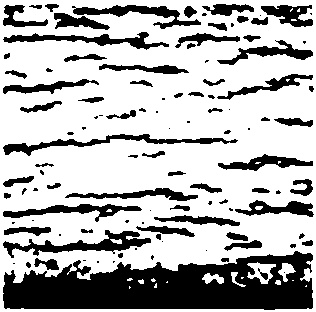
\includegraphics[width=0.4\textwidth]{Figures/blurred}\label{fig:blur_notblur2}}
		\caption{Comparison between Figure \ref{fig:blur_chu1} which has been thresholded, both with and without the application of a Gaussian blur algorithm (un-optimised inputs).}
		\label{fig:blur_notblur}
	\end{figure}
	
	The Gaussian blur is typically used to smooth boundaries in an image where an immediate change in pixel intensity is observed compared to neighbouring pixels. The function typically employs a square matrix of values known as a \textit{kernel}. This kernel is 'superimposed' over the individual pixel values by an algorithm in a \textit{raster} pattern and alters their intensity accordingly.
	
	\[
	\frac{1}{16}
	\begin{bmatrix} 
		1 & 2 & 1 \\
		2 & 4 & 2\\
		1 & 2 & 1 \\
	\end{bmatrix}
	\longrightarrow
	\begin{bmatrix}
		0 & 10 & 170 & 220 & 130 & 30 & 10\\
		0 & 12 & 180 & 241 & 122 & 35 & 14\\
		2 & 13 & 176 & 237 & 134 & 43 & 7\\
		2 & 13 & 174 & 236 & 129 & 40 & 7\\
		1 & 11 & 159 & 224 & 132 & 31 & 5\\
		0 & 13 & 178 & 242 & 136 & 44 & 9\\
	\end{bmatrix}
	\]
	
	The above example depicts a 3$\times$3 Gaussian blur kernel, although larger dimensions such as 5$\times$5 may also be used. The binary image (represented here by a 7$\times$6 matrix of pixel intensities) is \textit{convoluted} through a specific matrix operation. This alters the pixel intensities of the filtered image as weighted by the values in the kernel. There are two possible ways to adjust the level to which the image is filtered; by increasing the dimensions of the kernel, which increases the range over which the intensities are averaged, or by adjusting the values in the kernel to provide a greater or letter degree of filtering. Each route provides its own merits and drawbacks.
	\\
	
	\subsubsection{Gaussian blur methodology}
	In the context of this report, both routes to alter the Gaussian mask were trialled. The method proposed by S. Khan involved using a module named \textit{OpenCV}, which is a cross-platform open source module that focuses on image processing techniques such as as greyscale to binary conversion, Gaussian and median blurring, filtering and thresholding. One approach of clarifying hydrides in the zirconium matrix was to initially blur and remove noise from the image followed by application of a pixel filter value as a method of binarising (i.e. identifying a threshold value between 0 and 255). The idea behind this approach was to allow a user to specify threshold and kernel blur values by calling a single function, \textit{image\_conv}, which would display a clear binarised image with applied Gaussian blur. A before and after histogram is also displayed to show how the previous 8-bit image is filtered to a binary image with 0 and 255 as integer values. Image blur was increased by altering the dimensions of the mask overlaying the micrograph image. This served to significantly reduce the noise observed in Figure \ref{blur_notblur1}, however the method relies primarily on an odd-integer input to specify square dimensions of 1,3,5..., etc. This can reduce the versatility of the technique as it limits control over the amount of blurring achieved for a specific region of pixels. 
	\\
	\\
	A. Hanson proposed a similar technique but instead utilising the \textit{Scikit image} or \textit{skimage} package. In this method the values within the Gaussian blur are adjusted through the use of altering the standard deviation from the mean used by the filter. Here, a larger specified value for $\sigma$ will produce a larger range of values within the kernel and generate a more intense blurring, whilst lower $\sigma$ values will generate higher \textit{relative} pixel intensities at the fringes of the kernel and thus reduce the level of blurring, see Figure \ref{fig:chu1gauss} (after binary thresholding). It was thought that this method proposed was more suited for the purpose of this study, as python code written in skimage allowed the gaussian blur $\sigma$ to be adjusted individually for each image. So this was the approach taken forward.
	
	Here a function carries out the gaussian blur on an image array that has been read into python via \textit{skimage}, then the sigma values from the middle column of Table \ref{tab:imageprocessing} are specified in each case. There was also an additional input, \textit{truncation} value, which truncates the gaussian filter after the set amount of standard deviations. This was kept at a constant value of 3 throughout the study, as this was the default value recommended in skimage and also data within $3\sigma$'s accounts for 99.9\% of the data concerned. An example of this effect can be seen in Figure \ref{fig:blur_chu1}, as applied to the image from Figure \ref{fig:tem_hydride_eg}. After this, images were ready for binary thresholding in the next function.
	
	\begin{figure}[H]
		\centering
		\subfloat[Image 'chu1' filtered using a Gaussian mask where $\sigma$=0.5]{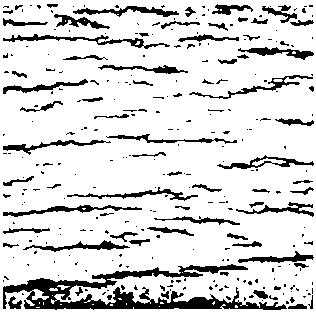
\includegraphics[width=0.4\textwidth]{Figures/chu1_s05_t04.jpg}\label{chu1_s05_t04}}
		\hfill
		\subfloat[Image 'chu1' filtered with $\sigma$=1.]{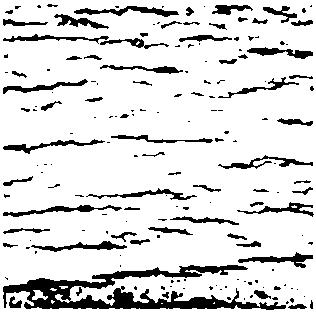
\includegraphics[width=0.4\textwidth]{Figures/chu1_s10_t04.jpg}\label{fig:chu1_s10_t04}}
		\caption{Post-processing of the same micrograph with differing values for $\sigma$. It is evident that higher values of $\sigma$ remove a larger quantity of noise between hydrides, but also result in aliasing of hydride boundaries and systematic removal of some regions.}
		\label{fig:chu1gauss}
	\end{figure}
	
	\subsection{Binary thresholding}
	Applying the same parameters in a Gaussian filter to different images tends to yield largely different results for the quantity of noise reduction in a range of images. In the sample image set provided for this investigation, many optical micrographs exhibited a high degree of peripheral darkening, which leads to difficulties in applying an effective intensity threshold without suffering losses to the visible hydrides. As such, a threshold and standard deviation must be manually agreed upon for each image to ensure maximum hydride retention whilst eliminating a sufficient quantity of noise. This presents a significant limitation of the approach as large quantities of micrographs may become time-intensive to analyse. In addition, the systematic removal of small hydride regions may generate a significant source of error when cross-comparing images. Practically, this can cause an over- or underestimation of hydride quantity within a sample and difficulties may arise in subsequent connectivity analysis.
	\\ 
	\\
	For the sample set of images; \textit{chu1, chu2, chu3, chu7, chu11}, threshold and filter values (namely $=\sigma$) were agreed upon based on their perceived effectiveness as follows. This series of images was selected, as they provided a series of different hydride morphologies for analysis. Thresholding is a very simple operation when done manually, it was applied with a simple python function that reads in the previously blurred image array, plots a respective histogram of it's pixel intensity values, and then applies the following operation, based on the specified threshold;
	\begin{center}
		In respective image array: $ value > threshold = true $
	\end{center}
	This sets any values in the image array greater than said threshold to true, numpy in python is then able to interpret this and convert this to an integer array of 1's and 0's which produces the binary images as displayed further on. In this case, a value of 1 is equal to white, when read in by skimage. An example of what this would look like in the code is displayed in Figure \ref{skbinary}.
	
	\begin{figure}[h]
	    \centering
	    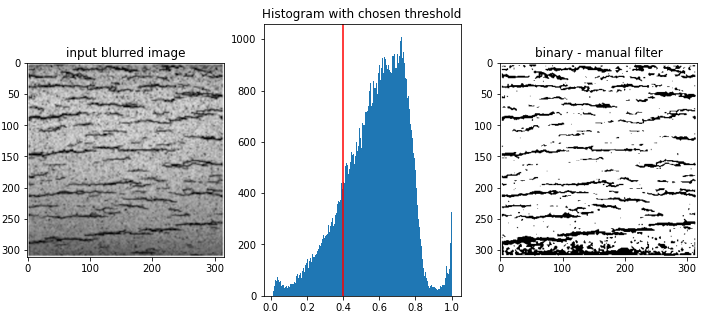
\includegraphics[scale=0.5]{Figures/chu1_skbinary.png}
	    \caption{A screenshot of the binary thresholding function output with selected threshold and intensity histrogram, as applied to chu 1. Dimensions of the image in pixels can be seen.}
	    \label{skbinary}
	\end{figure}
	
	With the manual approach in python, threshold values could be experimented with by simply running the written code, viewing the histogram and going back to change the threshold to a more optimal value appropriately. However this is subjective, parameters were chosen based on what was deemed to be best for the application. A number of other threshold methods were investigated in skimage before choosing the manual approach, though it was found that these were too difficult to optimise for the purpose and the simple manual method was sufficient. Examples of different binary filters can be seen in Figure \ref{fig:skimage_threshold} in the appendix.
	\\
	\\
	Two sets of parameters were selected for each image conversion to highlight the effect of gaussian blurring and thresholding on the output images. This was done after some experimentation to find the appropriate range of values to find a satisfactory output image. As such, the images filtered with the lower set of values are referred to as \textit{low-pass} (LP) and those filtered through higher values are denoted \textit{high-pass} (HP), see Table \ref{tab:imageprocessing}.Examples of all these output images can be seen in Figure \ref{fig:combined_thresholds} for comparison purposes.
	
	\begin{table}[ht]
	\begin{center}
	\begin{tabular}{ |c|c|c|c| } 
		\hline
		\multicolumn{4}{|c|}{Low-pass Images} \\
		\hline
		Image Reference & $\sigma$ (Gaussian blur) & Intensity Threshold Value & Gaussian Truncation Value \\
		\hline
		\textit{chu1} & 0.5 & 0.4 & 3 \\ 
		\textit{chu2} & 0.5 & 0.35 & 3 \\ 
		\textit{chu3} & 0.5 & 0.5 & 3 \\ 
		\textit{chu7} & 1.0 & 0.4 & 3 \\ 
		\textit{chu11} & 1.0 & 0.4 & 3 \\ 
		\hline
	\end{tabular}
	\\
	\begin{tabular}{ |c|c|c|c| } 
		\hline
		\multicolumn{4}{|c|}{High-pass Images} \\
		\hline
		Image Reference & $\sigma$ (Gaussian blur) & Intensity Threshold Value & Gaussian Truncation Value \\
		\hline
		\textit{chu1} & 1.0 & 0.5 & 3 \\ 
		\textit{chu2} & 1.0 & 0.4 & 3 \\ 
		\textit{chu3} & 1.0 & 0.4 & 3 \\ 
		\textit{chu7} & 1.0 & 0.6 & 3 \\ 
		\textit{chu11} & 1.0 & 0.5 & 3 \\ 
		\hline
	\end{tabular}
	\caption{Tested parameters gaussian blur $\sigma$ and binary threshold (see later sections) for the studied images using the \textit{scikit image} approach. This was split into low-pass and high-pass to investigate the effect of altering parameters.}
	\label{tab:imageprocessing}
	\end{center}
	\end{table}
	
    These values generated the following pre-processed images shown in Figure \ref{fig:combined_thresholds}. It can be seen that the HP images have introduced much more noise and darkened areas, which warps the size of the hydrides - losing some definition. Due to this it was decided to proceed to analysis with the low-pass binary images produced in an effort to reduce both excessive noise and excessive hydride omission.

	\begin{figure}[H]
		\centering
		\subfloat[\textit{chu1(LP)}: $\sigma$=0.5, T=0.4]{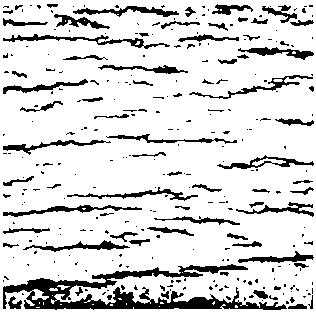
\includegraphics[width=0.4\textwidth]{Figures/chu1_binary3_sigma05_thres04.jpg}\label{chu1LP}}
		\hfill
		\subfloat[\textit{chu1(HP)}: $\sigma$=1.0, T=0.5]{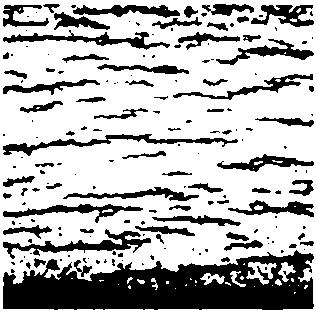
\includegraphics[width=0.4\textwidth]{Figures/chu1_binary1_sigma1_thres05.jpg}\label{chu1HP}}
		\label{fig:chu1LPHP}
		\subfloat[\textit{chu2(LP)}: $\sigma$=0.5, T=0.35]{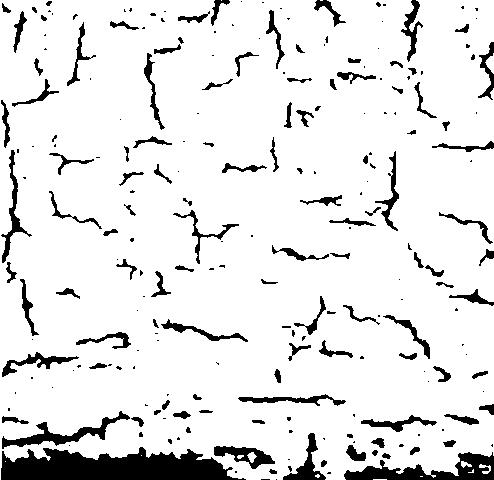
\includegraphics[width=0.4\textwidth]{Figures/chu2_binary3_sigma05_thres035.jpg}\label{chu2LP}}
		\hfill
		\subfloat[\textit{chu2(HP)}: $\sigma$=1.0, T=0.4]{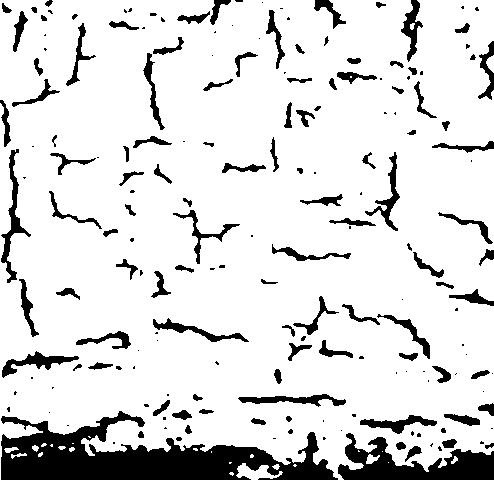
\includegraphics[width=0.4\textwidth]{Figures/chu2_binary1_sigma1_thres04.jpg}\label{chu2HP}}
		\label{fig:chu2LPHP}
		\subfloat[\textit{chu3(LP)}: $\sigma$=1.0, T=0.4]{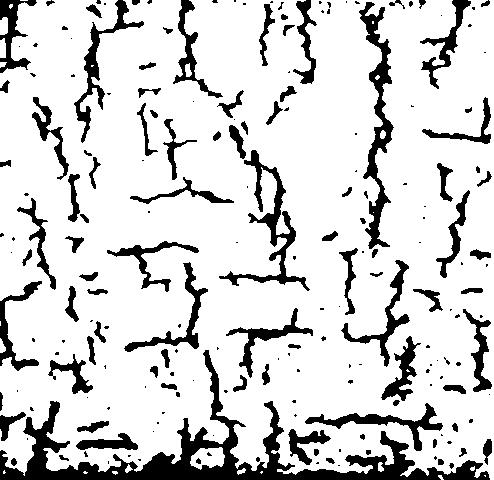
\includegraphics[width=0.4\textwidth]{Figures/chu3_binary1_sigma1_thres04.jpg}\label{chu3LP}}
		\hfill
		\subfloat[\textit{chu3(HP)}: $\sigma$=0.5, T=0.5]{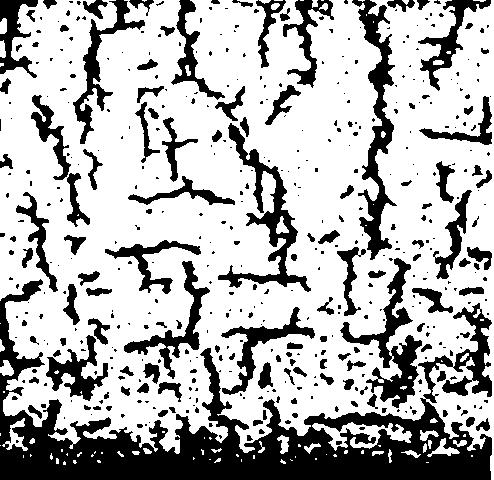
\includegraphics[width=0.4\textwidth]{Figures/chu3_binary1_sigma05_thres05.jpg}\label{chu3HP}}
		\label{fig:chu3LPHP}
	\end{figure}
	\begin{figure}[H]
		\centering
		\subfloat[\textit{chu7(LP)}: $\sigma$=1.0, T=0.4]{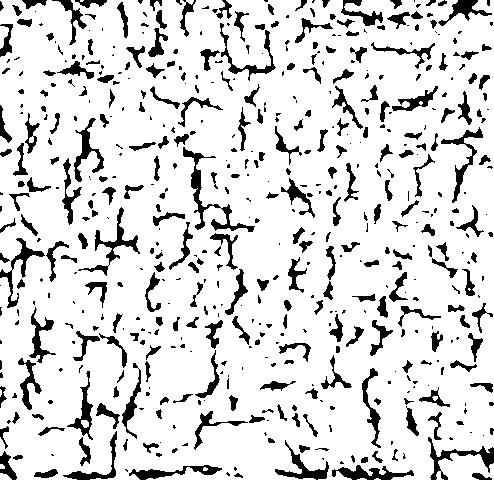
\includegraphics[width=0.4\textwidth]{Figures/chu7_binary1_sigma1_thres04.jpg}\label{chu7LP}}
		\hfill
		\subfloat[\textit{chu7(HP)}: $\sigma$=1.0, T=0.6]{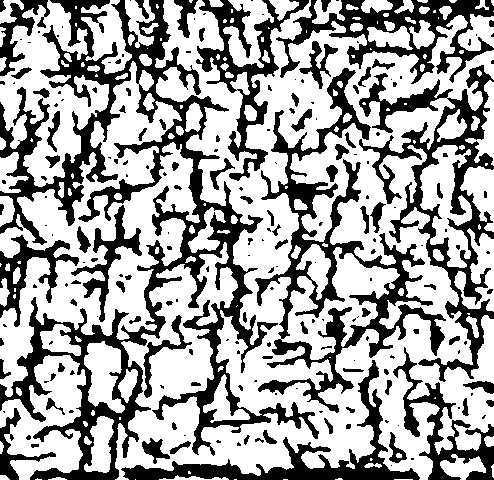
\includegraphics[width=0.4\textwidth]{Figures/chu7_binary2_sigma1_thres06.jpg}\label{chu7HP}}
		\label{fig:chu7LPHP}
		\centering
		\subfloat[\textit{chu11(LP)}: $\sigma$=1.0, T=0.4]{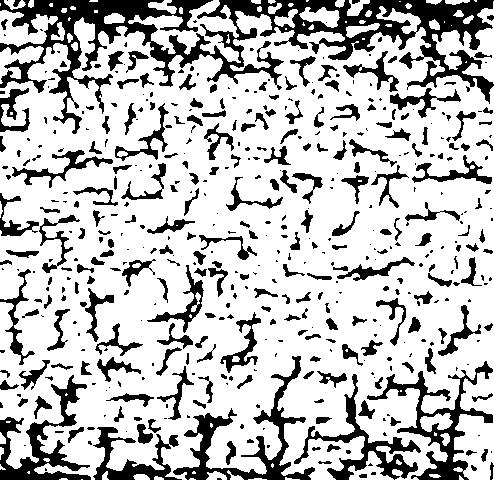
\includegraphics[width=0.4\textwidth]{Figures/chu11_binary1_sigma1_thres04.jpg}\label{chu11LP}}
		\hfill
		\subfloat[\textit{chu11(HP)}: $\sigma$=1.0, T=0.5]{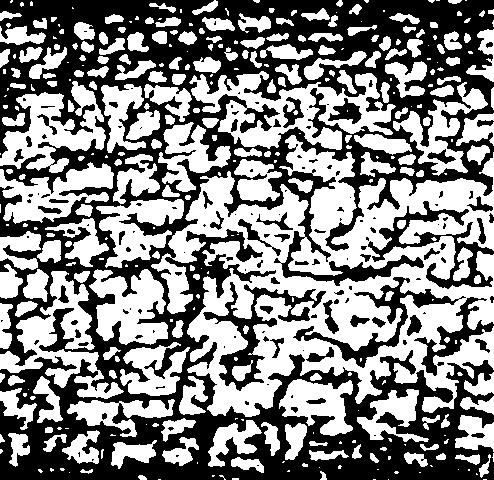
\includegraphics[width=0.4\textwidth]{Figures/chu11_binary3_sigma1_thres05.jpg}\label{chu11HP}}
		\label{fig:chu11LPHP}
		\caption{Pre-processed micrographs from the sample image set. Two images with differing threshold and $\sigma$ values are included for each micrograph.}
		\label{fig:combined_thresholds}
	\end{figure}

	\section{Initial Trial Methods to Assess Hydride Connectivity}
	Following pre-processing, techniques were trialled in an attempt to analyse the level of connectivity between regions of H\textsubscript{4}Zr in the micrographs \cite{Simon2021}\cite{Sharma2018}\cite{Sunil2020}.

	\subsection{Skeletonise function from Sci-kit Image}
	Skeletonisation was implemented as an initial approach for obtaining a simplified path for connected hydrides. This function would theoretically reduce the hydride map to a connected graph of thin lines (approximately one pixel in thickness). Using \textit{skimage.morphology}, the skeletonise() function was tested on image ‘chu1’. From the demo code produced, an initial reading of the file from the local directory was performed followed by specifying the image size. Using \textit{skblur} and \textit {skbinary}, ‘chu1’ was binarized and blurred to give the output as shown in Figure 4a. It is interesting to note that there were different variants to the skeletonise() function. One output (Zha84) initially takes the edges of an object (a hydride in this case) and iteratively removes pixels, stopping when the neighbouring pixel is black (where the intensity is zero) \cite{ScikitimageA}. As long as the image in Figure 4 (a) is inverted, the result is a series of single white pixel lines. Another output (Lee94) uses an 'octree' data structure which is more suitable for 3D images. Like Zha84, this algorithm also performs sweeping iterations over the image where pixels are continuously removed until the condition is satisfied where two iterations produce the same image and there is no change in the pixel count \cite{ScikitimageA}. Figure ~\ref{Zha84}  and Figure~\ref{Lee94} shows the results of Zha84 and Lee94 methods respectively, which were applied to the binarised ‘chu1’image from Figure 4a.

	\begin{figure}[h]
		\centering
		\subfloat[Zha84 method of skeletonisation applied to 'chu1'.]{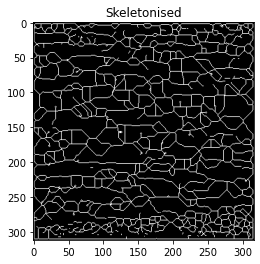
\includegraphics[width=0.4\textwidth]{./Figures/Skeletonised_Chu1}\label{Zha84}}
		\hfill
		\subfloat[Lee94 method of skeletonisation applied to 'chu1'.]{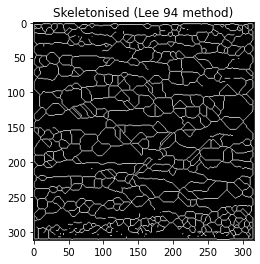
\includegraphics[width=0.4\textwidth]{./Figures/Skeletonised_Lee_Chu1}\label{Lee94_2}}
		\caption{Processing image 'chu1' with two skeletonisation methods. }
		\label{Skeletonise}
	\end{figure}

	These results, however, are unsuitable for analysing connectivity as it appears that the matrix has been identified as the object rather that the hydrides themselves. Crucially, the skeletonise function does not provide actual data which can be applied to find suitable microstructural characteristics. Therefore, it was decided to assess an alternative characteristic of the microstructure to determine the hydride characteristics (discussed later). Finally, Figure~\ref{MedialAxis} below illustrates a representation of how \textit{medial\_axis} works by identifying the edges of the hydrides and then prints a skeleton (colour map=magma) \cite{ScikitimageA}. In this case the skeleton is performed on the matrix rather than the hydride, this may be because of the initial ‘chu1’ binary image array, as these values are not inverted.
	\\
	\begin{figure}[h]
		\centering
		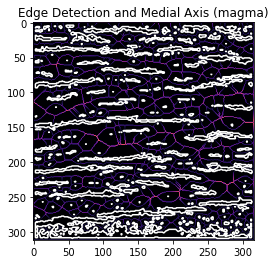
\includegraphics[width=2.5in]{Figures/Medial_Axis_Chu1} 
		\caption{Skeletonisation approach with medial axis pattern printed in a magma colour map, again applied to 'chu1'.}
		\label{MedialAxis}
	\end{figure}
	\\
	\subsection{Canny Edge Detection and the Hough Line Transform}
	
	The \textit{Hough Line Transform} relies on the detection of pixels within a series of lines superimposed onto a sample image. An algorithm is used to plot a series of lines for which pixels within a region may coincide. A greater 'intensity' is recorded for lines that coincide a larger number of pixels, and peaks are achieved for lines with the greatest intensities (i.e. the line corresponds to a roughly linear region of pixels). Rather than a typical first-order equation $y=mx+c$, the method defines these lines as the perpendicular normal to a line of angle $\theta$ from the top-left origin, of length $r$. This places pixel regions in the co-ordinate space $(r,\theta)$ ('Hough space') as opposed to traditional cartesian co-ordinates. This is advantageous as lines may then be separated according to different values of $\theta$, as is required to compute the radial hydride fraction.
	\\
	\begin{figure}[H]
		\centering
		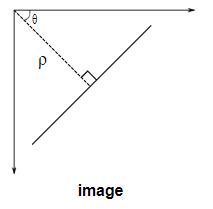
\includegraphics[width=2.5in]{Figures/houghtransform.PNG} 
		\caption{A single line is plotted of distance $\rho$ (defined in this report as $r$) from the origin in the upper left corner. The angle $\theta$ is used in conjunction with $\rho$ to discern the positon and orientation of the line, which is useful in calculating a RHF value for the sample \cite{OpenCV2013}.}
		\label{MedialAxis}
	\end{figure}
	It has been established that the Hough transform is useful in detecting shapes using mathematical forms such as cartesian coordinates. For the case of straight lines, Hough space can be used to identify the distance from the image origin to a line and the angle of the line relative to a specified axis. This description is for the OpenCV, \textit{cv2}, module which uses the ‘cv2.houghlines’ function. The main advantage of using Hough transform when put up against skeletonise is that it can return rho and theta values in a 2D array. Rho is the distance which is taken as positive if the line is above the origin and negative if the line is below the origin. Theta is the angle measured from the horizontal axis in the counter-clockwise direction. ‘Hough.transform’ uses the coordinate system (rho, theta) in a voting system \cite{OpenCV2013}. Here, a straight horizontal black line can be visualised in a white background image. If the start point of the line is at an initial value of (40, 90), ‘Hough.transform’ will detect this and begin searching the image to find matching the number of (40,90) cells. The maximum count for this cell would indicate that a line lies on this coordinate \cite{OpenCV2013}. When using the function, Canny edge detection was used to better visualise the hydrides. This function can also simply threshold and binarise an image, without allowing the user to change truncation or sigma values. After testing, the following results were given, as shown in Figure \_ (a) and (b).
	\\
	\begin{figure}[h]
		\centering
		\subfloat[Canny edge detection on image 'chu2']{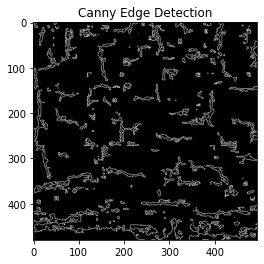
\includegraphics[width=0.4\textwidth]{./Figures/Canny_Edge_Detection}\label{Canny}}
		\hfill
		\subfloat[Attempted Hough transform on image 'chu2']{\includegraphics[width=0.4\textwidth]{./Figures/Hough_Transform_chu2}\label{Lee94}}
		\caption{Canny edge detection and hough.transform() used on image 'chu2' taken from Figure 4c. }
		\label{Skeletonise2}
	\end{figure}
	\\
\pagebreak
\section{Radial Hydride Fraction to Assess Connectivity}
\subsection{Initial Approach using Hough Line Transform}

    Due to difficulties in implementing a viable technique for determining the level of connectivity of hydrides within test micrographs, the focus of the project was adjusted to assist in determining the likelihood of through-wall cracking and subsequent mechanical failure of analysed zirconium samples. As previously highlighted, the rate of degradation of fuel cladding is dependent on the orientation of hydrides within the grains. However as observed many samples exhibit hydrides oriented both radially and circumferentially; a ratio is therefore needed to assess the contributions of the hydride orientations to the likelihood of failure by through-wall cracking. Known as the \textit{Radial Hydride Fraction} (RHF) and discussed previously, this provides a measure of the proportion of hydrides oriented perpendicular to the hoop direction, thus constituting a greater risk of through-wall cracking within the sample. RHF can be loosely related to the likelihood of failure of a cladding element as the formation of radial hydrides (known as \textit{hydride reorientation}) is associated with the quantity of hydrogen within the structure as well as the circumferential orientation of stress fields, both of which are a consequence of high irradiation fluence and exist in fuel assemblies at high burnup levels \cite{Plyasov2020}. As such, samples exhibiting these effects pose a greater risk of compromise to their structural integrity.
    \\
    \\
    Simon et al. 2021 \cite{Simon2021} comprehensively discussed RHF, and defined it as a widely used metric to quantify hydride morphology with many specific formulas. Though generally it may be expressed as defined by Colas at el. 2013 \cite{Colas2013}:
    
    \begin{equation}
        RHF = \frac{ \sum_i{L_i f_i} }{ \sum_i{L_i} }
    \end{equation}
    \label{equ:RHF}
    
    Where $f_i$ is:
    
    \begin{equation}
        f_i = 0; 0^{\circ} \leq \theta \leq 40^{\circ},\hspace{1cm} or = 0.5;  40^{\circ} \leq \theta \leq 65^{\circ}, \hspace{1cm} or = 1.0; 65^{\circ} \leq \theta \leq 90^{\circ}
    \end{equation}
    
    Theta corresponds to the angle relative to the circumferential direction, where $\theta = 0^{\circ}$, is said direction and $\theta = 90^{\circ}$ would be the radial direction. A limitation here is that since the metric does not differentiate between hydrides between these angle ranges, some morphologies may be classified as having the same RHF and the same behaviour. Though as this report seeks to qualitatively assess hydride connectivity with image processing in a simple manner, more advanced classification may be out of the scope of this study.
    \\
    \\
    With this, a method then needs to be pursued which is able to object size or length and the angle of said object in respect to either axis or direction. This could be done by implementing the \textit{straight line hough transform}, as discussed \cite{ScikitimageB}, and \textit{measure} packages in Skimage. 
    \\
    \\
    Initially a python function was developed named \textit{"hough\_measure"} which would take an input binary array, label "objects" using binary criteria in respect to the background and then perform a hough transform on these objects. The transform was always set to take place between angles $\frac{-\pi}{2}$ and $\frac{\pi}{2}$, the lines in hough space would then be plotted in terms of distance in pixels against the respective angles, producing a number of sinusoidal functions where the \textit{hough peaks} would be displayed (these are the areas that obtain the higher number of counts or votes). From this, python would then be able to interpret these peaks and plot out the respective detected hough peak lines back onto the input binary image, this should theoretically then correspond to the "connected" regions of hydrides in the image and provide corresponding angles and sizes. Such an output is shown as it would appear in python in Figure \ref{fig:hough_initial}. The function had many inputs, however they will not be discussed in detail yet as immediately a number of issues were identified in this initial hough transform approach (which is seen in the figure).
    
    \begin{figure}[H]
        \centering
        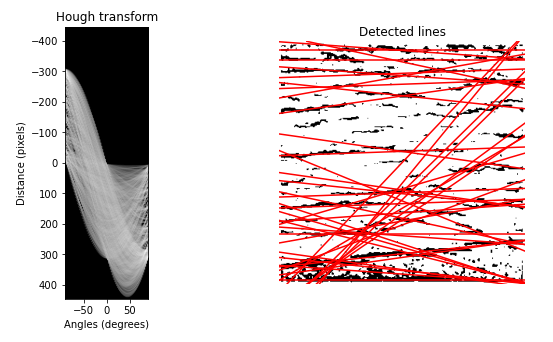
\includegraphics[scale=0.7]{Figures/houghtrans_initial.png}
        \caption{An example of "hough\_measure function as applied to Chu 1. It can be seen on the left that the hough peaks are difficult to identify, there are no clear brightspots (possibly due to too many peaks). Additionally on the right, many lines have been plotted and some do not seem logical.}
        \label{fig:hough_initial}
    \end{figure}
    
    Figure \ref{fig:hough_initial} shows that many potential hough lines were plotted on the first binary image; some of these lines are expected and map possible hydride paths, however other lines are clearly illogical and plot an unexpected connectivity or morphology. It is possible from the output that too many hough peaks were generated, meaning that there would be a large amount of lines plotted. In this case, not all lines have been plotted due to some limiting conditions such as minimum separating distance and angle, though it does imply that overall there were too many peaks calculated. Additionally, this approach has no way to assess individual hydride morphology or direction, only the direction and angle of the "most likely" line passing through many hydrides. So there is no way to apply the methodology from equation \ref{equ:RHF}.
    
    This shows that taking a hough transform over an entire labelled image in python is not appropriate, and the image must be broken up or individual objects must be isolated for proper analysis.
   

\subsection{Refined Approach}
\textbf{Modified hough transform function using slicing}
    
    
    To tackle the issue with isolating hydrides using skimage hough transform methodology, inspiration was given by Maric et al., 2021 \cite{Maric2021}. This approach uses has the same function as  described previously, though extra capability is added with \textit{SciPy ndimage} \cite{Scipy2021}. Using Scipy the labelled objects in a binary image from \textit{skimage measure} could be sliced around and treated as a separate variable in the array. Using for loops and indexing, it is then possible to carry out a hough transform on each individual identified object. This meant that each object could be identified with a boundary rectangle, and then hough peak lines could be plotted within this rectangle, which would be isolated from other objects, meaning individual hydride morphologies could be assessed. This function was named \textit{hough\_measurebox}.
    \\
    \\
    The inputs for the \textit{hough\_measurebox} function are summarised in Table \ref{HoughmeasureboxInputs}. As there were many input parameters, it was decided that it would be best to have a standardised input for a reliable comparison between the resulting radial hydride fractions. As changing multiple inputs would make it impossible to make a proper comparison without extensive investigation. These inputs are based on documentation read in \cite{ScikitimageB}, which provides default and recommended values. More on the basis of choosing these is listed below:

    \begin{itemize}
        \item \textit{Minimum distance between lines} - Adjusting this within the same order of magnitude seemed to have minimal effect, but it was not investigated in-depth.

        \item \textit{Minimum angle between lines} - This seemed suitable. It has a major effect on resulting output, but changing this would need further investigation.

        \item \textit{Fraction} - (Minimum peak intensity) It was found that 0.5 was too high, as this would eliminate objects less than 50\% size of the maximum detected object in said slice. This may reduce some key lines.

        \item \textit{Peak number} - This introduces large deviations in the detected lines and results, as it decides how many peaks are plotted for the given hough transform in each slice. The largest are always plotted first. 5 seemed appropriate
    \end{itemize}

    \begin{table}[h]
	    \begin{center}
	    \begin{tabular}{ |c|c|c| } 
		    \hline
		    \multicolumn{3}{|c|}{\textbf{hough\_measurebox Inputs}} \\
		    \hline
		    \textbf{Function Input} & \textbf{Value} & \textbf{Basis for Chosen Input} \\
		    \hline
		    \textit{Background value} & 1 & Always set to white. \\
		    \hline
		    \textit{Minimum distance between lines} & 5 & The default skimage value, seems suitable. \\ 
		    \hline
		    \textit{Minimum angle between lines} & 5 & The default in skimage, assumed to be degrees. \\
		    \hline
		    \textit{Fraction} & 0.3 & The default is 0.5 in skimage. \\ 
		    \hline
		    \textit{Peak number} & 5 & The default value is assumed maximum in skimage. \\ 
		    \hline
	    \end{tabular}
	    \caption{Inputs for the slicing hough line transform function in python, used for the analysis of each image.}
	    \label{HoughmeasureboxInputs}
	    \end{center}
    \end{table}
    
    Using these inputs, \textit{hough\_measurebox} is able to provide a series of angles (in degrees) and sizes (in pixels) for each hydride slice, these can be concatenated into lists and stacked into an array. The resulting output is then an array of angles and heights, corresponding to every hydride detected according to the input. An example of what this looks like in python is displayed in Figure \ref{fig:houghmeasure_chu1}.
    
    \begin{figure}[h]
        \centering
        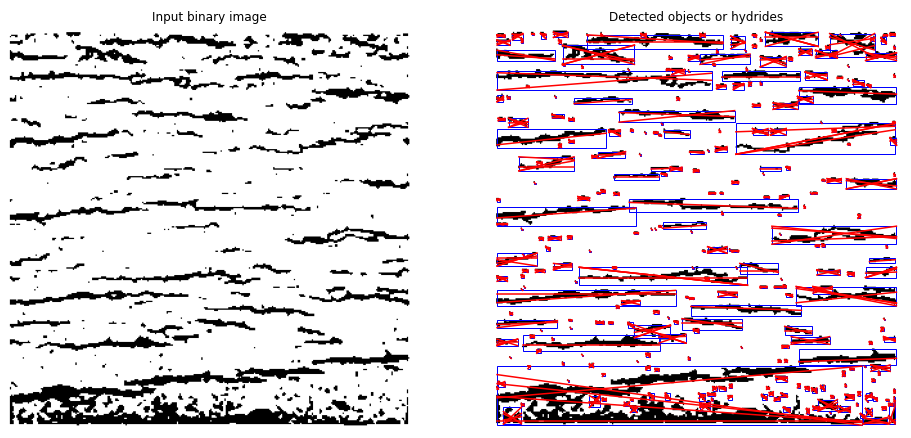
\includegraphics[scale=0.5]{Figures/houghmeasure_chu1.PNG}
        \caption{The \textit{hough\_meaurebox} output for chu 1, boxes can be seen plotted around the detected objects as according to skimage.measure label and the hough peak lines are plotted for the specified inputs (Table \ref{HoughmeasureboxInputs}).}
        \label{fig:houghmeasure_chu1}
    \end{figure}
    
    To then analyse this output and calculate the respective RHF's, the criteria discussed earlier from \ref{equ:RHF} would have to be effectively reversed; as the angles from the hough transform are taken in respect to the y-axis (which is the radial direction in a hydride). This is a simple case of reversing the criteria:
    
    \begin{equation}
        f_i = 0; 65^{\circ} \leq \theta \leq 90^{\circ},\hspace{1cm} or = 0.5;  40^{\circ} \leq \theta \leq 65^{\circ}, \hspace{1cm} or = 1.0; 0^{\circ} \leq \theta \leq 40^{\circ}
    \end{equation}
    
    This again implemented by writing a python function, that would perform equation \ref{equ:RHF} on the array of angles and heights. This function would then provide a radial hydride fraction (to 2 decimal places) and a maximum and minimum hydride size in pixels, which can be discussed in each case.
    
\subsection{Implementing Automatic Testing}
    In order to learn how to implement automatic testing using GitHub and Python, and to check reliability of the analysis of the code in this study, automatic testing was implemented. This was done using the Python Application GitHub action in Git workflows, utilising the \textit{pytest} package. As it is difficult to automatically test the image processing steps of the study, it was thought to assess the the analysis of RHF as this is a quantity that can be somewhat predicted. So a methodology was proposed to produce a number of "test hydride" images which had a known radial hydride fraction, or in this case approximately estimated based on the previously explained criteria of RHF. Figures \ref{TestImages64} and \ref{TestImage300} below shows the test images created.

    \begin{figure}[H]
		\begin{center}
		\subfloat[Test image 1, 64 by 64 pixels, with 3 radially orientated false hydrides]{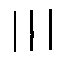
\includegraphics[width=0.2\textwidth]{./Figures/Test_1.jpg}
		\label{TestImage1}}
		\hspace{6pt} 
		\subfloat[Test image 2, 64 by 64 pixels, Test Image 1 rotated by 90 degrees]{
\includegraphics[width=0.2\textwidth]{./Figures/Test_2.jpg}
		\label{TestImage2}}
		\caption{The first test hydride images produced of 64 by 64 pixel size.}
		\label{TestImages64}
		\end{center}
	\end{figure}

    \begin{figure}[H]
        \begin{center}
        
\includegraphics[width=2.0in]{Figures/Test_3.jpg} 
        \caption{Test image 3, 300 by 300 pixels, with a single circumferential hydride.}
        \label{TestImage300}
        \end{center}
    \end{figure}

    The test images were produced in ImageJ software, setting the background as white (a value of 255 when read into skimage) and the fake hydrides as black (0). The first 2 images were set to image size of 64 pixel squares, with approximately 40 pixel object lengths (these were drawn on with angles 90\textdegree and 0\textdegree respectively). The third image was created in the same manner, except its size was set to 300 by 300 pixels, as this is closer to the sample micrograph images assessed in the study. This image had only 1 fake hydride of 260 pixel length. These images should have Radial hydride fractions of 1.0, 0.0 and 0.0 respectively if the code functions as it should and detects only these singular objects in the hough transform.
    \\
    \\
    Based on this, a testing procedure was proposed which sets a number of criteria that pytest would be able to test the images against using the \textit{assert} command. For \textbf{Test image 1}, a wholely radially orientated image, this cycled through:

    \begin{center}
        Test 1: $assert\:RHF > 0.8$ \newline
        Test 2: $assert\:RHF > 0.9$ \newline
        Test 3: $assert\:RHF == 1.0$ \newline
    \end{center}

    For \textbf{Test images 2 and 3}, similar criteria were set but reversed as the fake hydrides were orientated in the circumferential direction, as follows:
    \begin{center}
        Test 1: $assert\:RHF < 0.2$ \newline
        Test 2: $assert\:RHF < 0.1$ \newline
        Test 3: $assert\:RHF == 0.0$ \newline 
    \end{center}

    These criteria would allow users to see if a test image fell into the expected RHF range depending how it is orientated, and then finally it can be checked to see if the function is truly accurate by assessing whether RHF is equal to 1.0 or 0.0.  However before doing this the images must be pre-processed similarly to the micrographs analysed in the study, which means running them through \textit{skblur} and \textit{skbinary} in the test code. To minimise the effect that these may have, they were run with specified inputs shown in Table \ref{tab:TestImageTable}. A Gaussian blur sigma and binary threshold of 0 is used, to produce no blurring and to set any image objects to binary pixels.

    \begin{table}[h]
        \centering
        \begin{tabular}{|c|c|}
        \hline
            \textbf{Function parameter} & \textbf{Test image input}  \\
            \hline
            $\sigma$ (Gaussian blur) & 0.0 \\
            \hline
            Gaussian Truncation Value & 3 \\
            \hline
            Intensity Threshold Value & 0.0 \\ 
        \hline
        \end{tabular}
    \caption{Test image pre-processing parameters used for \textit{skblur} and \textit{skbinary}.}
    \label{tab:TestImageTable}
    \end{table}

    After this, testing could be implemented with the criteria as explained above in each case. A separate test .py file was made for each test image, and then whenever the testing reposity was pushed or a pull request was created, the test workflow would run.

\section{Results and Discussion}
\subsection{Radial Hydride Fractions with Standard Inputs}
    The resulting radial hydride fractions and hydride sizes for each analysed image (low pass condition, Figure \ref{fig:combined_thresholds}) are shown in Table \ref{tab:RHF_results}. It can be seen that despite what was thought to be a large variation in hydride morphology and definition, the overall RHF's do not vary outside of the range of 40\%-60\% and this could be for a number of reasons. Figure shows the output of hough transform python function for each of the LP binary images from Figure \ref{fig:combined_thresholds}.

    \begin{table}[ht]
	    \begin{center}
	    \begin{tabular}{ |c|c|c|c| } 
		    \hline
		    \textbf{Image Reference} & \textbf{RHF} & \textbf{Minimum object size (pixels)} & \textbf{Maximum object size (pixels)} \\
		    \hline
		    \textit{chu1} & 0.24 & 1.0 & 267.0 \\
		    \hline
		    \textit{chu2} & 0.43 & 1.0 & 245.0 \\
		    \hline
		    \textit{chu3} & 0.54 & 1.0 & 491.0 \\ 
		    \hline
		    \textit{chu7} & 0.57 & 1.0 & 76.0 \\ 
		    \hline
		    \textit{chu11} & 0.46 & 1.0 & 394.0 \\ 
		    \hline
	    \end{tabular}
	    \caption{Results of the radial hydride fraction analysis of each tested image, according to inputs of Table \ref{Houghmeasureboxinputs}}
	    \end{center}
	    \label{tab:RHF_results}
    \end{table}

    \begin{figure}[H]
		    \centering
		        \subfloat[\textit{Hough Transform Analysed Chu 1 (repeated from Figure \ref{fig:houghmeasure_chu1} for clarity)}]{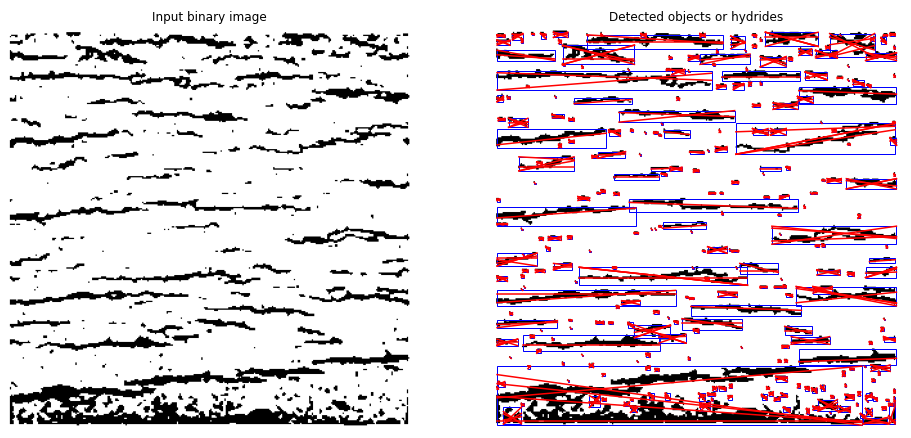
\includegraphics[scale=0.4]{Figures/houghmeasure_chu1.PNG}\label{chu1hough}}
		        
		        \subfloat[\textit{Hough Transform Analysed Chu 2}]{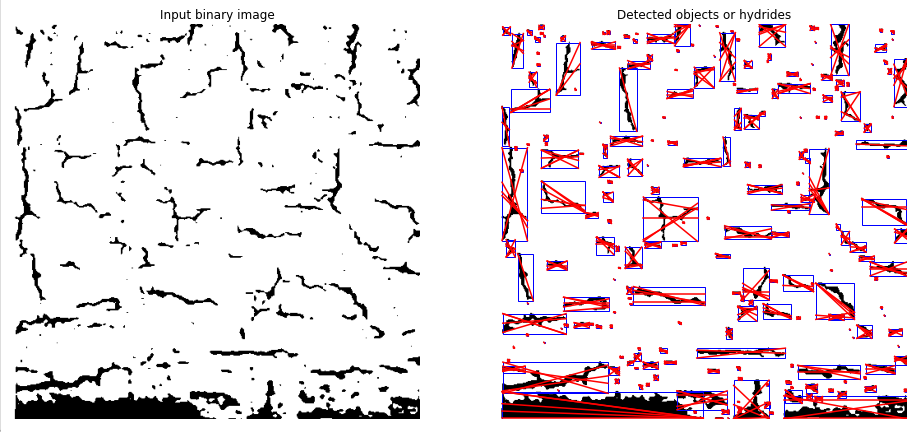
\includegraphics[scale=0.4]{Figures/houghmeasure_chu2.PNG}\label{chu2hough}}
		        
		        \subfloat[\textit{Hough Transform Analysed Chu 3}]{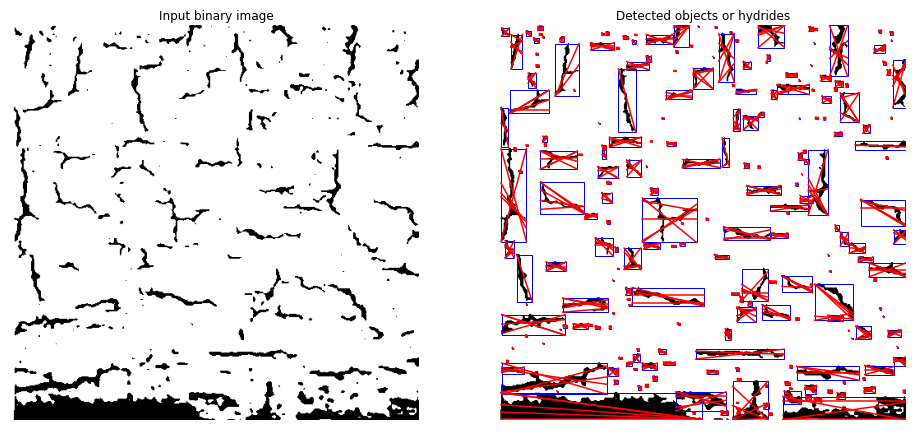
\includegraphics[scale=0.4]{Figures/houghmeasure_chu3.PNG}\label{chu3hough}}
		        
		        \subfloat[\textit{Hough Transform AnalysedChu 7}]{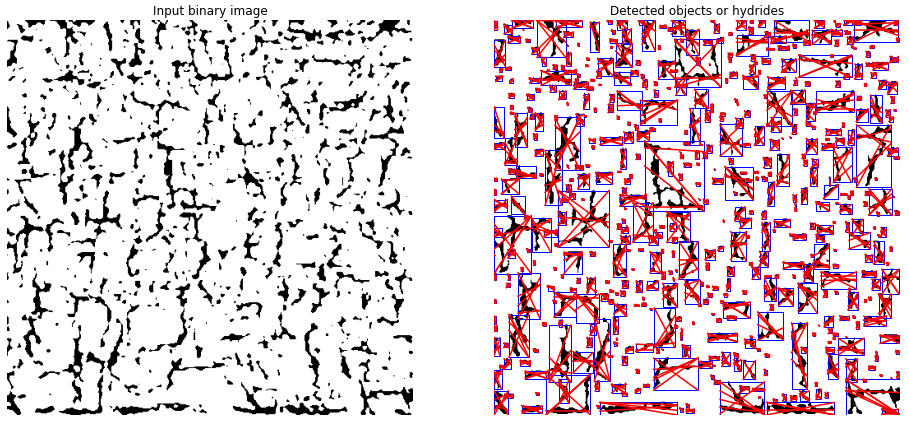
\includegraphics[scale=0.4]{Figures/houghmeasure_chu7.PNG}\label{chu7hough}}
		        
		        \subfloat[\textit{Hough Transform Analysed Chu 11}]{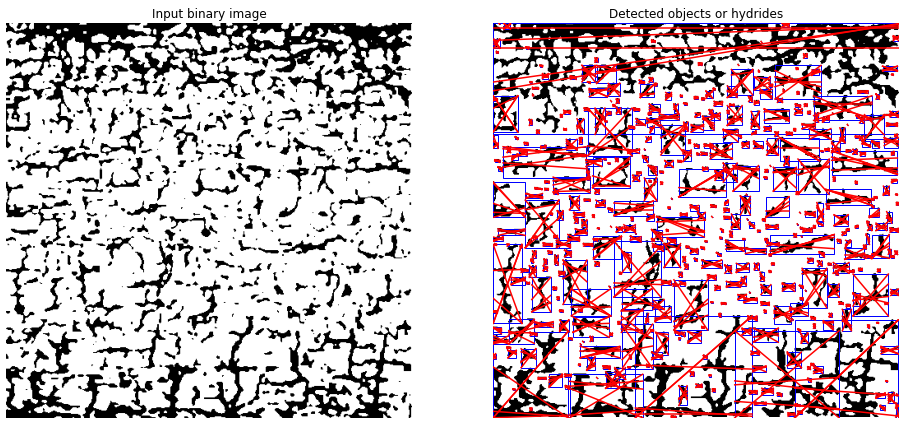
\includegraphics[scale=0.4]{Figures/houghmeasure_chu11.PNG}\label{chu11hough}}
	        \caption{The output of \texit{hough\_measurebox.py} on all binary images from Figure \ref{fig:combined_thresholds}, using the inputs specified in Table \ref{HoughmeasureboxInputs} for the RHF analysis.}
	        \label{fig:RHF_results_all}
	\end{figure}

    \textbf{SOME NOTES}
    \begin{itemize}
        \item pre-processing stages work effectively and provide useable .
        \item Noise consideration - top and bottom images, darkened effect from microscope view or from image processing stages.
        \item \textbf{Noise as top \& bottom of image does influence results - larger objects are created and detected as being large hydrides.}
        \item \textbf{WHAT DO WE SAY ABOUT THE RESULTING RHF'S, SIZES ETC., ALL RESULTS ARE NOW HERE}
        \item Chu 7 and 11 have a similar proportion of radial and circumferential orietnated hydrides, so do chu 2 and 3 - so perhaps we'd expect similiar values
        \item There is a clear difference between all of them and Chu 1.
        \item In hindsight, another fully circumferential and fully radially orientated hydride should've been analysed (polarised morphology).
        \item In hindsight, should have included a small object removal stage.
        \item In Chu 3, there is significant darkening in the bottom which has created a large connected object which is then taken by the code as fully radial ~ this may heavily impact the results (despite some radially orientated hydrides can be seen nearby).
        \end{itemize}

\subsection{Influence of Peak Number on Radial Hydride Fraction}

    The peak number is the main input in skimage hough transform package that decides how many hough line peaks will be plotted and shown in the output data. It was thought that performing a small investigation on the effect of adjusting this may be useful in learning more about the limitations of RHF and the python code written. Image 3 (chu 3), provides a complex mixed morphology and was thought to be a good candidate to assess this, though image 1 (chu 1) was also thought to be worth trying. Table \ref{tab:peakno_tests} shows the results of what was attempted, peak numbers 2 and 10 were used in comparison with a peak number of 5 as used in the main results.

    \begin{table}[h]
        \centering
        \begin{tabular}{|c|c|c|}
        \hline
        \multicolumn{1}{|l|}{\textbf{Image Reference}} & \textbf{Peak Number} & \textbf{RHF} \\ \hline
        \multirow{}{}{\textit{Chu 1}}                & 2                    & 0.56         \\ 
                                                      & 10                   & 0.54         \\ \hline
        \multirow{}{}{\textit{Chu 3}}                & 2                    & 0.13         \\ 
                                                      & 10                   & 0.32         \\ \hline
        \end{tabular}
        \caption{The influence of adjusting peak number on RHF, in the case of images 1 and 3.}
        \label{tab:peakno_tests}
    \end{table}
    
    \begin{figure}[H]
        \centering
        \subfloat[Peak number = 2]{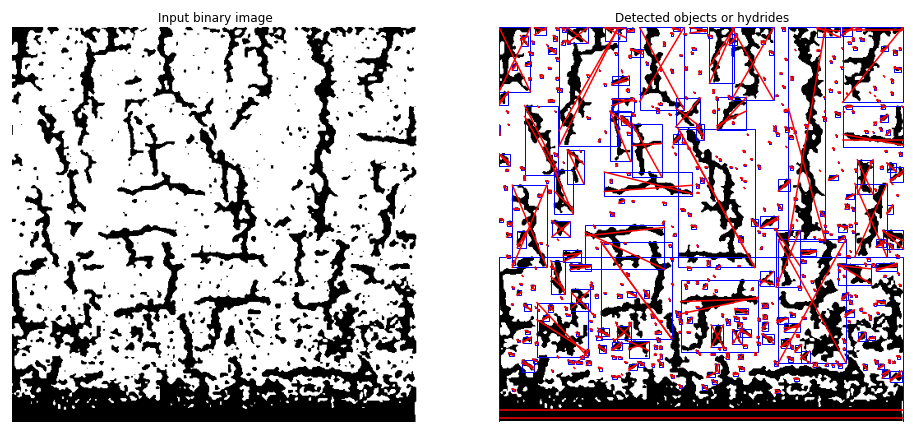
\includegraphics[scale=0.5]{Figures/houghmeasure_chu3_PN2.PNG}}
        \hfill
        \subfloat[Peak number = 10]{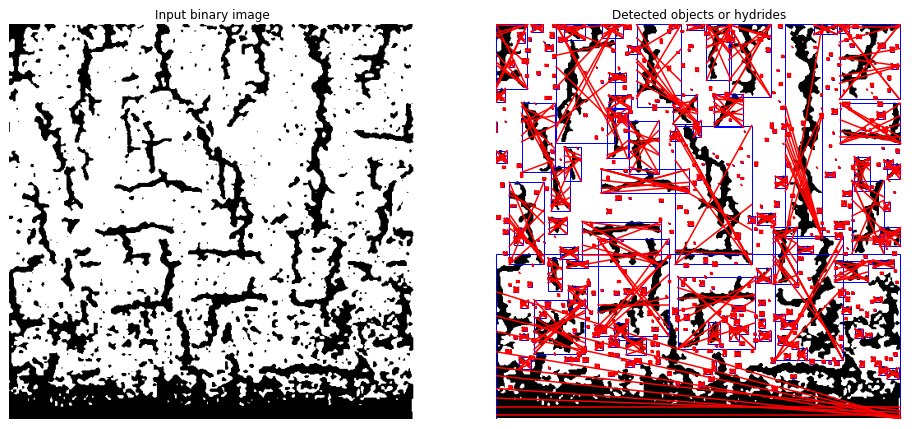
\includegraphics[scale=0.5]{Figures/houghmeasure_chu3_PN10.PNG}}
        \caption{Chu 3 analysed as describe in regards to Table \ref{tab:peakno_tests} .}
    \label{fig:chu3_PN_comparison}
    \end{figure}
    
    It can be seen that in the case of Chu 3 a peak number reduction only has a slight effect, increasing the RHF by 0.02 (only a marginal increase). Perhaps this may imply that larger hydrides are dominant in this case (which is expected), as there is still a midpoint between radial and circumferentially aligned hydrides which are being assessed in image 3 and hence the 56\% RHF. With limited peaks, only the predominant hough peaks are plotted for each slice (which tends to be the larger objects). However, we can see that many small objects are still being assigned their own slice and being analysed, which is an issue with the code and would require greater image processing steps to remove these smaller objects.
    
    When peak number is increased Many lines appear as expected, and the overall the directions of each seem very undetermined, they pass through a number of objects in a slice but may not necessary have an overall large contact length, somewhat reflecting what was seen with the old hough line transform function (Figure \ref{fig:hough_initial}). This does not seem to influence the RHF significantly though, as it has only decreased by 0.01 (1\%). This further reinforces the point from above, with larger hydrides having more influence on the analysis.
    \\
    \\
    A problem is introduced when looking at the effect of changing peak number on Chu 1, here it seems to have a major effect in each case. Decreasing peak number to 2 does seem to lower RHF to 0.13 (from 0.24 with 5 originally), which implies that larger hydrides take a more dominant role. However increasing peak number to 10, shifts RHF upwards to 0.32 meaning that the micrograph effectively becomes more radially orientated despite this is not the case (recall Figure \ref{fig:houghmeasure_chu1}). Looking back at the image output, it is possible that the many smaller objects are being heavily factored into the RHF calculation, or lines of different directions that could be detected on the larger hydrides. For example, at the bottom of Chu 1 is a larger darkened area of noise which is treated as a huge object, more radially orientated lines could possibly be plotted on this. The overall amount of smaller objects being interpreted in radial orientation may actually have an increasing effect on the overall RHF of the image, as each object has its own slice with lines within according to the peak number. This further confirms that improvements need to be made in the image processing stages. 
    
\subsection{Automatic Testing; Pytest Results}
    The output of the tests produced by the Git workflow as summarised in Table \ref{TestResults}.

    \begin{table}[h]
        \centering
        \begin{tabular}{|c|c|c|}
        \hline
            \textbf{Test Image} & \textbf{Tests Passed} & \textbf{Output RHF From Testing}  \\
            \hline
            1 & 3/3 & 1.0 \\
            \hline
            2 & 1/3 & 0.13 \\
            \hline
            3 & 2/3 & 0.01 \\
            \hline
        \end{tabular}
        \caption{The output of the automatic testing with pytest on GitHub using test images.}
        \label{TestResults}
    \end{table}

    It can be seen from the results, that only Test image 1 was able to pass all tests. Test images 2 and 3 failed some of the criteria. This is made obvious when looking at the output RHF in Table \ref{TestResults}. Test image 2 shows an unexpected result, and Test image 3 has some marginal error and is 1\% out from the expected value. This is not a major concern for Test image 3, as it is approximately correct (though the code does not recognise this), however for Test image 2 these is quite a high margin of error with RHF being approximately 13\% greater than expected. In order to verify what this may, the images were run through the python functions manually using inputs from Table \ref{tab:TestImageTable} to see the hough transform output. This is shown in Figure \ref{TestImagesProcessed} for Test images 2 and 3.

    %I cant seem to get latex to detect these figures but they are in the right area?
    \begin{figure}[h]
        \centering
        \subfloat[Test image 2 processed]{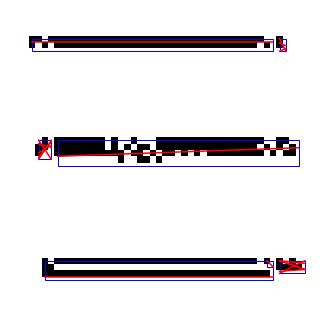
\includegraphics[width=0.4\textwidth]{Figures/test2_processsed.png}}
        \hfill
        \subfloat[Test image 3 processed]{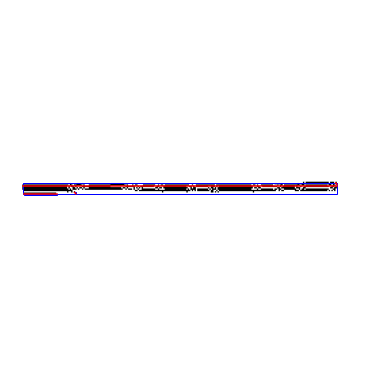
\includegraphics[width=0.4\textwidth]{Figures/test3_processsed.png}}
        \caption{Test images run through hough\_measurebox using default inputs, some noise is seen from the binary thresholding which highlights a problem.}
    \label{TestImagesProcessed}
    \end{figure}

    One of the image processing stages (likely the binary thresholding stage, as gaussian blurring was eliminated using $\sigma$=0) has generated some \textit{noise} or \textit{pixel artefacts} on the fake hydride objects in the images. This can be seen in both images, Figure \ref{TestImagesProcessed} a and b, of 64 and 300 square pixel size. However, it has had a larger effect on the smaller image, as any introduced small objects from noise or error will have greater effect. In Test image 2, there are 2 smaller objects which have been effectively broken off the main objects by the noise which leads to smaller hydrides which could be orientated in any direction according to the code. This could lead the hough transform to interpret these as being aligned perpendicular to the intended test hydride direction (circumferential), hence there is a deviation in the RHF leading to the error. In Test image 3, this has had a very slight effect due to the main object size dominating RHF, hence it has only deviated by ~1\%. 

    These observed effects however do highlight a major problem in the image processing binary threshold stage or the nature of the test, which could be an effect of simple manual thresholding. In this case the threshold was set to 0, and as values of true black in hex code or RGB code (from ImageJ) are all 0's, this should have been interpreted as 0 in \textit{skblur} and \textit{skbinary} and the threshold applied on any non-black pixels. Here some pixels were obviously interpretted as greater than 0 despite they should be read as 0 values. 
    \\
    \\
    This may have been an issue with the image production method using ImageJ drawing software, to verify this, Test Image 2 was read into \textit{skbinary} manually and the histogram was observed, it displayed that there was a small distribution of values around pixel intensity 0 and 255, not just the 2 polarised values. So the threshold was set properly in the next case, each object could then be fully "binarised". This was then implemented to the automatic test using new pre-processing parameters as shown in Table \ref{tab:TestImageTable2}.
    
    \begin{table}[h]
        \centering
        \begin{tabular}{|c|c|}
        \hline
            \textbf{Function parameter} & \textbf{Test image input}  \\
            \hline
            $\sigma$ (Gaussian blur) & 0.0 \\
            \hline
            Gaussian Truncation Value & 3 \\
            \hline
            Intensity Threshold Value & 0.1 \\ 
        \hline
        \end{tabular}
    \caption{Test image pre-processing parameters used for \textit{skblur} and \textit{skbinary} in the secondary test.}
    \label{tab:TestImageTable2}
    \end{table}
    Following on from this change, all test were able to pass with the following results in Table \ref{TestResults2} . This verifies that the code should be working correctly to calculate RHF, despite there was some doubts about the resulting RHF's from the real sample micrographs in the results section.
    
    \begin{table}[h]
    \centering
    \begin{tabular}{|c|c|c|}
    \hline
        \textbf{Test Image} & \textbf{Tests Passed} & \textbf{Output RHF From Testing}  \\
        \hline
        1 & 3/3 & 1.0 \\
        \hline
        2 & 3/3 & 0.0 \\
        \hline
        3 & 3/3 & 0.00 \\
        \hline
    \end{tabular}
    \caption{The output, after amending binary threshold, of the automatic testing with pytest on GitHub using test images.}
    \label{TestResults2}
\end{table}
    
    There is drawbacks to this testing approach, as the test images have to be viewed, read in and analysed manually first to see what threshold and blurring parameters should be applied to "optimise" their condition for the hough line transform and RHF analysis tests. This partially eliminates the purpose of the automatic testing, and it may introduce some bias to the testing parameters. It is thought that it may have been better to set up a test with default or expected parameters first, view the outcome and then attempt to learn and adjust code from there as opposed to the former. It would also be better to carry out testing on more complex morphology test micrographs, however this introduces issues with estimating and predicting RHF before the test. This however does highlight opportunities for future work in the area regarding the binary thresholding method and further automatic testing with python and git workflows.

\section{Conclusions}
\subsection{On Hydride Structure Analysis}

\subsection{Recommendations}
\begin{itemize}
    \item Image processing could be more optimised, i.e. a small object removal stage, and there should be an extensive investigation into threshold selection as it was perhaps not optimised well.
    \item Each input parameter (refer to table) of the hough line transform 
    
    \item correlate RHF with mechanical properties or embrittlment
    \item RHF could be linked to actual longetivity of the sample, to make a practical link (or crack likelihood?)
    \item additional pre-processing to remove dark fringes? Skikit-image offers package 'NiBlack'
\end{itemize}


\newpage
\bibliographystyle{abbrv}
\bibliography{References}

\newpage
\appendix
\section{Additional figures}

\begin{figure}[h]
	    \centering
	    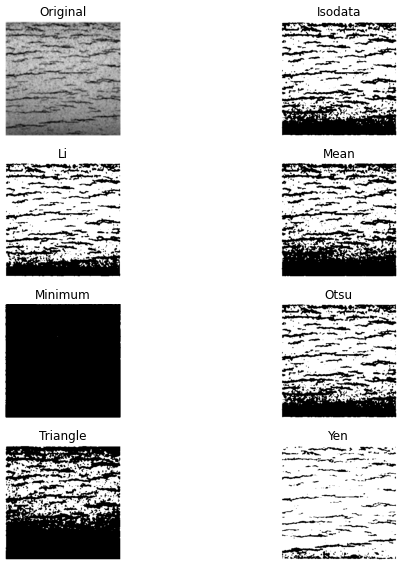
\includegraphics[scale=0.7]{Figures/skimage_thresholds.png}
	    \caption{A range of binary thresholds that were applied in the skimage package to Chu 1, overall these were difficult to optimise and some generated excess noise.}
	    \label{fig:skimage_threshold}
	\end{figure}
	
\section{Individual Reflections}
\subsection{Jake the potato harvester}
Your contribution to the project
war'gwan dickheads my drilla big al in the house spitting bars in your grill, tell your gyal to buss me her snapchat fam
Talk to my g sully for top bants and kek you dusty yute

How successful you think it was

How would you address the project differently
\subsection{Sulayman the Magnificent}

\subsection{A. Hanson}
Alexander the Great
code works
lel
one pound hydride
very very good and very very cheap
come on ladies
come on ladies
one pound hydride
\end{document}
